% ============================================================
% ICAIS 2026 Track 2: Young Scientist | 4-Page Compact
% Spectral Immunity: A Frequency-Domain Reliability Audit
% Framework for Physics-Derived Outputs in AI Scientists
% Final Version v9 - With All Review Fixes
% ============================================================
\documentclass[9pt,twocolumn]{article}

% ============ Basic Packages ============
\usepackage[UTF8]{ctex}
\usepackage[english]{babel}
\usepackage{amsmath,amssymb,amsfonts}
\usepackage{amsthm}
\usepackage{booktabs}
\usepackage{multirow}
\usepackage[font=scriptsize,labelfont=bf,skip=0pt]{caption}
\usepackage[hidelinks,colorlinks=true,linkcolor=black,citecolor=black,urlcolor=black]{hyperref}
\usepackage[margin=1.3cm,columnsep=0.45cm,top=1.6cm,bottom=1.1cm]{geometry}
\usepackage{setspace}
\usepackage{fancyhdr}
\usepackage{float}
\usepackage{enumitem}
\usepackage{titlesec}
\usepackage{array}
\usepackage{xcolor}
\usepackage{mathtools}
\usepackage{bm}
\usepackage{graphicx}
\usepackage{algorithm}
\usepackage{algpseudocode}

% ============ Theorem Environments ============
\newtheorem{proposition}{Proposition}
\newtheorem{theorem}[proposition]{Theorem}
\theoremstyle{remark}
\newtheorem{remark}[proposition]{Remark}
\theoremstyle{definition}
\newtheorem{definition}[proposition]{Definition}

% ============ Page Setup ============
\setlength{\parindent}{0.5em}
\setlength{\parskip}{0pt}
\renewcommand{\baselinestretch}{0.68}
\setlength{\abovecaptionskip}{0.5pt}
\setlength{\belowcaptionskip}{0pt}
\setlength{\floatsep}{1pt}
\setlength{\textfloatsep}{1pt}
\setlength{\intextsep}{1pt}
\setlength{\abovedisplayskip}{0.5pt}
\setlength{\belowdisplayskip}{0.5pt}
\setlength{\abovedisplayshortskip}{0.3pt}
\setlength{\belowdisplayshortskip}{0.3pt}

\pagestyle{fancy}
\fancyhf{}
\fancyhead[L]{\scriptsize\itshape ICAIS 2026 Track 2: Young Scientist}
\fancyhead[R]{\scriptsize\thepage}
\renewcommand{\headrulewidth}{0.2pt}
\setlength{\headheight}{14pt}
\setlength{\headsep}{5pt}

\titleformat{\section}{\normalsize\bfseries}{}{0em}{}
\titlespacing{\section}{0pt}{0.5pt}{0.2pt}
\titleformat{\subsection}[runin]{\small\bfseries}{}{0em}{}
\titlespacing{\subsection}{0pt}{1pt}{1pt}

\setlist{nosep,leftmargin=*,itemsep=0pt,topsep=0pt}

% ============ Custom Commands ============
\newcommand{\pxrmse}{\sigma_{\text{px}}}
\newcommand{\physerr}{\epsilon_{\text{phys}}}
\newcommand{\nprf}{\text{NPRF}}
\newcommand{\snf}{S_n(f)}
\newcommand{\hsysf}{|H_{\text{sys}}(f)|^2}
\newcommand{\Hsqmean}{\overline{H^2}}
\newcommand{\Beff}{\mathcal{B}_{\text{eff}}}

% Compact algorithm setup
\makeatletter
\newcommand{\algorithmiccompact}{\renewcommand{\algorithmicrequire}{\textbf{Input:}}\renewcommand{\algorithmicensure}{\textbf{Output:}}}
\makeatother

\begin{document}

\twocolumn[
\vspace{-6pt}
  \begin{center}
    {\Large\bfseries Spectral Immunity: A Frequency-Domain Reliability Audit Framework for Physics-Derived Outputs in AI Scientists}

    \vspace{2pt}

    {\small\bfseries Submitted to ICAIS 2026 Track 2: Young Scientist}

    \vspace{3pt}

    {\small Rosslyn Yang \ \ Ethan Lin \ $^{1}$}

    \vspace{0.5pt}

{\scriptsize $^{1}$ Nankai High School, Tianjin, China \quad \texttt{mdrosslyning@gmail.com} \quad \texttt{daoming\_kan@163.com}\quad Supervisor: Wei Teng}
    \vspace{0.5pt}

    {\scriptsize\textbf{Human Responsibility Statement:} Core scientific insights, all theorem derivations, experimental design and analysis are completed independently by the authors. AI tools are only used for Python code syntax debugging and English abstract polishing. All experimental codes and data are fully reproducible.}

    \vspace{0.5pt}
    \rule{\linewidth}{0.4pt}
  \end{center}
]

% ==================== Abstract ====================
\section*{Abstract}
\vspace{-1pt}
\begingroup
\scriptsize
\setlength{\parindent}{0.8em}

Reliability evaluation for AI-Scientist systems still relies on pixel-level RMSE. Its implicit assumption---that observation-space precision proxies physical-space accuracy---which we term the \textbf{pixel hallucination}, systematically fails for physics-derived outputs. When the error power-spectral density is non-flat within the resonant frequency band of physical operators, under a fixed pixel RMSE $=10^{-3}$, the ratio of physical error between white-noise and red-noise inputs reaches 3.03-fold. This paper proposes the \textbf{Spectral-Immunity framework}. Its core metric, the Normalized Physical Risk Factor (NPRF), takes white noise as the baseline. Given only spectral estimation of AI output residuals and one-off offline calibration of the operator frequency response, NPRF automatically computes spectral health during inference without requiring ground-truth physical values.

Experiments reveal: (1) Under fixed pixel RMSE $=10^{-3}$, white noise yields 153.5\% physical error while red noise yields only 50.7\%; (2) Under amplitude-controlled conditions, NPRF achieves a Spearman rank correlation of 0.968 against physical error, forming complementary diagnostics alongside RMSE; (3) An early-warning case study shows two models with \textit{identical} pixel RMSE ($0.00200$) but physical errors differing by 8.26-fold (98.7\% vs.\ 815.3\%), correctly flagged by NPRF ($0.113$ vs.\ $8.875$); (4) Residual spectra of standard-MSE-trained models are dominated by signal frequency structures rather than training-noise type. Ablation experiments confirm a large effect from the 60 Hz component ($p=0.000042$, Cohen's $d=1.558$); training-noise-type effects are \textit{not} statistically significant after Bonferroni correction ($p=0.056$, power $\approx0.35$), warranting larger samples; (5) Standard Butterworth low-pass filtering degrades NPRF by 380.0\% under non-stationary noise; (6) Post-hoc spectral reshaping via five-stage notch filtering reduces NPRF by 49.8\% and physical error by 31.0\% ($p=0.001953$) without retraining; (7) A preliminary real-world experiment on basketball projectile motion obtains NPRF$=0.177$ (workflow demonstration only; $N=53$ insufficient for statistical inference).

\vspace{0.2pt}
\noindent\textbf{Keywords:} AI-for-Science; spectral reliability; NPRF; physical-quantity derivation; spectral immunity

\endgroup

\vspace{0.2pt}
\hrule
\vspace{0.2pt}

% ==================== 1. Introduction ====================
\section{Introduction}

\subsection{An Overlooked Problem}

From 2023 to 2024, AI-Scientist systems achieved breakthroughs in protein-structure prediction (AlphaFold 3\cite{abramson2024}), materials discovery (GNoME\cite{merchant2023}), and global weather forecasting (GraphCast\cite{lam2023}). Their shared workflow accepts observational data and outputs physical quantities via deep networks. Nevertheless, one fundamental problem has been systematically ignored: \textbf{how can an AI scientist judge whether its physically-derived outputs are reliable?}

This paper focuses on reliability auditing for the workflow below:

\begin{equation}
\label{eq:workflow}
\text{Observed data} \xrightarrow{\text{AI model}} \hat{\mathbf{x}} \xrightarrow{\text{physical derivation operator}\ \mathcal{D}} \hat{a}
\end{equation}

Here $\hat{\mathbf{x}}$ denotes the AI output in observation space; $\mathcal{D}$ is a deterministic operator for deriving physical quantities (differentiation, deconvolution, integral transforms). Pixel-level RMSE evaluates error in the first stage, whereas credibility of physical experiments depends on errors of the second-stage output $\hat{a}$. Huge gains within specific frequency bands from the frequency response of $\mathcal{D}$ may amplify the mapping between these two spaces by orders of magnitude.

Within conventional scientific practice, human researchers perform cross-validation via replicated experiments, alternative methodologies, and theoretical expectations. When AI takes over these steps, reliability assessment is simplified to pixel-wise RMSE. This embeds an untested proxy assumption: precision in observation space can proxy accuracy in physical space. We name this unquestioned acceptance the \textbf{pixel hallucination}, and prove that this assumption fails systematically.

\textbf{Why AI-Scientists specifically require this.} In autonomous laboratories\cite{burger2020}, AI-Scientists generate hypotheses, design experiments and interpret results in closed loops; when evaluators contain spectral blind spots, errors are written into knowledge bases undetected. Deep networks fit high-frequency components more slowly than low-frequency ones\cite{xu2019,rahaman2019,tancik2020,ronen2019}; residual spectra are intrinsically non-flat. AlphaFold\cite{abramson2024} predicts hundreds-of-millions protein structures within months; even a 1\% spectral-blind-spot error rate exceeds the total errors made by human scientists across lifetimes. \textbf{Spectral immunity is thus a core component of AI-Scientist metacognition.}

\textbf{Scope.} This paper does not propose a new AI model. Instead, it addresses: \textit{when an AI model outputs physical quantities, how can the AI system itself know whether those outputs are trustworthy?} We provide the diagnostic tool (NPRF), the early-warning demonstration (Exp.\ 2b), and the remedy (post-hoc reshaping).

\subsection{Related Work}

Spectral bias is well-documented: deep networks fit low-frequency components first\cite{rahaman2019,xu2019,tancik2020,ronen2019}. Classical UQ (Bayesian\cite{kendall2017}, ensembles\cite{lakshminarayanan2017}) asks ``how uncertain?'' not ``how physically dangerous?'' SG differentiation\cite{savitzky1964} amplifies high-frequency noise, but no prior work connects operator frequency response to AI-pipeline reliability auditing. We fill this gap.

\subsection{Physical-Ground-Truth Sandbox (PGTS)}

We construct a \textbf{Physical-Ground-Truth Sandbox (PGTS)}: constant-acceleration trajectories ($a_{\text{ref}}=9.8$ m/s$^2$), with accelerations derived by a 21-point third-order Savitzky-Golay filter\cite{savitzky1964}. The SG filter's combined frequency-response squared magnitude $\hsysf$ exhibits a resonant peak at $f_{\text{peak}}=51$ Hz; the theoretical noise-amplification factor is $\sqrt{\sum_{i=1}^{21} c_i^2}=13353.3$. A tracking system with pixel residual RMSE $10^{-3}$ thus yields derived acceleration RMSE up to $13.35$ m/s$^2$, corresponding to 136.3\% relative physical error. The measured 153.5\% for white noise reflects SG boundary effects at finite signal length.

\subsection{Contributions}

Both authors contributed equally. (1) \textbf{Diagnostics} (\S 2.1): prove proxy metrics valid iff error PSD is flat across the operator's effective passband. (2) \textbf{Tool} (\S 2.2): propose NPRF, requiring no physical ground truth. (3) \textbf{Early-warning} (\S 3.3): demonstrate NPRF flags 8.26-fold physical-error disparity undetectable by pixel RMSE. (4) \textbf{Remedy} (\S 3.5): validate post-hoc spectral reshaping.

% ==================== 2. Spectral-Immunity Theory ====================
\section{Spectral-Immunity Theory}

\subsection{Spectral Adversarial Vulnerability}

Consider noisy trajectories $\hat{\mathbf{x}} = \mathbf{x} + \mathbf{n}$, with noise PSD $\snf$. Define:
\begin{equation}
\label{eq:metrics}
\pxrmse = \sqrt{\mathbb{E}[(\hat{x}_i - x_i)^2]}, \quad \physerr = \frac{\text{RMSE}(\hat{a}, a_{\text{ref}})}{|a_{\text{ref}}|} \times 100\%.
\end{equation}

\begin{definition}[Spectral-Adversarial Vulnerability]
Let physical quantities be derived by linear operator $\mathcal{D}$ with combined transfer function $H_{\text{sys}}(f)$. If two noise processes satisfy $\pxrmse^{(1)}=\pxrmse^{(2)}$ yet $\physerr^{(1)}\neq\physerr^{(2)}$, the evaluation pipeline exhibits \textbf{spectral-adversarial vulnerability}.
\end{definition}

\begin{theorem}[Sufficiency Condition for Proxy-Metric Validity]
\label{thm:sufficiency}
Suppose $\mathcal{D}$ is linear time-invariant with combined squared frequency response $\hsysf$. Fix threshold $\theta \in (0,1)$. Define the \textit{effective passband}:
\begin{equation}
\label{eq:band}
\Beff(\theta) = \bigl\{f \in [0, f_s/2] : \hsysf \geq \theta \cdot \max_{f'} \hsysf \bigr\},
\end{equation}
where $|\Beff|$ denotes Lebesgue measure. If noise PSD $\snf$ satisfies: \textbf{(i) effective-support condition}---$\exists \epsilon>0$ such that $\int_{f \notin \Beff} \hsysf \,\snf \, df \leq \epsilon \int_{\Beff} \hsysf \,\snf \, df$ and $\int_{f \notin \Beff} \snf \, df \leq \epsilon \int_{\Beff} \snf \, df$; \textbf{(ii) approximate flatness condition}---$\exists S_0>0, \delta>0$ such that $\sup_{f \in \Beff} |\snf - S_0|/S_0 \leq \delta$. Then there exists $C(\theta)$ depending only on $\mathcal{D}$, $\theta$, $f_s$ such that
\begin{equation}
\label{eq:thm_bound}
\bigl|\physerr - C(\theta) \cdot \pxrmse \bigr| = O(\delta + \epsilon),
\end{equation}
where $C(\theta) = \frac{1}{|a_{\text{ref}}|} \sqrt{\frac{\int_{\Beff} \hsysf \, df}{|\Beff|}}$. \textit{Proof:} By Parseval's identity\cite{brillinger2001}, $\operatorname{Var}[\hat{a}] = \int_{0}^{f_s/2} \hsysf \,\snf \, df$; result follows from (i)--(ii) by direct substitution.
\end{theorem}

\begin{remark}[Intuitive interpretation]
Theorem~\ref{thm:sufficiency} says: \textbf{if the noise spectrum is approximately flat across the operator's effective passband, pixel RMSE is a good proxy for physical error.} Red noise (low-frequency) makes RMSE \textit{overestimate} risk; resonant-band noise makes RMSE \textit{underestimate} risk. $\theta$ typically $10^{-3}$--$10^{-6}$. For non-linear systems, first-order Taylor local linearization applies; the theorem provides intuition rather than a tight bound. For practical purposes, NPRF (\S 2.2) serves as the operational metric without requiring threshold selection.
\end{remark}

\subsection{Normalized Physical Risk Factor (NPRF)}

\begin{theorem}[Spectral Variational Principle for Physical Error]
\label{thm:variational}
Subject to $\int \snf \, df = \pxrmse^2$ and $\snf \geq 0$, a tight upper bound for physical-quantity variance is $\pxrmse^2 \cdot \max_f \hsysf$. Equality iff $\snf$ is a Dirac-$\delta$ at $\arg\max_f \hsysf$.
\end{theorem}

\textbf{From passband to full-band normalization.} Unlike Theorem~\ref{thm:sufficiency}'s passband-restricted analysis, NPRF uses the full-band arithmetic mean of $\hsysf$ as the normalization baseline. This choice is analytically tractable (no threshold $\theta$ to select), directly interpretable (white noise $\Rightarrow$ NPRF$=1$), and robust to operator types whose effective passband may be multimodal or ill-defined.

Define the \textbf{Normalized Physical Risk Factor (NPRF)}:
\begin{equation}
\label{eq:nprf_def}
\nprf = \frac{\int_{0}^{f_s/2} \hsysf \,\snf \, df}{\pxrmse^2 \cdot \Hsqmean},
\end{equation}
where $\Hsqmean = \frac{1}{f_s/2}\int_{0}^{f_s/2} \hsysf \, df$ is the arithmetic mean of $\hsysf$. \textbf{NPRF equals the ratio of the $\hsysf$-weighted average to the plain arithmetic average of $\hsysf$}, normalized to white-noise baseline. NPRF only requires Welch spectral estimation\cite{welch1967} of residuals plus one-off offline calibration; \textbf{no physical ground truth required}.

\textbf{Interpretation of ``normalized''.} NPRF is normalized \textit{relative to white noise}, not relative to safety. NPRF$=1.0$ = white-noise baseline, \textbf{not} a safety threshold (white noise at $\sigma_{\text{px}}=10^{-3}$ already yields 153.5\% physical error). NPRF $<1.0$ = safer than white noise given same pixel RMSE. Absolute risk:
\begin{equation}
\label{eq:decomposition}
\sigma_a = \pxrmse \cdot \sqrt{\Hsqmean \cdot \nprf}.
\end{equation}

\textbf{Deployment workflow.} The complete diagnostic procedure is summarized in Algorithm~1.

\begin{algorithm}[htbp]
\scriptsize
\algorithmiccompact
\begin{algorithmic}[1]
\Require AI residual $\mathbf{r}[n]$, calibrated operator response $\hsysf$, sampling rate $f_s$
\Ensure NPRF score and risk flag
\State Estimate PSD: $\snf \leftarrow \text{Welch}(\mathbf{r}, f_s)$ \Comment{$O(N\log N)$}
\State Compute pixel RMSE: $\pxrmse \leftarrow \text{std}(\mathbf{r})$
\State Compute normalization: $\Hsqmean \leftarrow \frac{1}{f_s/2}\int \hsysf \, df$
\State Compute NPRF via Eq.~\eqref{eq:nprf_def}
\If{$\nprf > 2.0$}
    \State Flag: ``HIGH spectral risk''; recommend Spectral-Immunity filter
\ElsIf{$\nprf > 1.5$}
    \State Flag: ``MODERATE spectral risk''; recommend inspection
\Else
    \State Flag: ``Low spectral risk (relative to white noise)''
\EndIf
\State \Return $\nprf$, flag
\end{algorithmic}
\caption{Spectral Immunity Check (deployment-ready)}
\label{alg:nprf}
\end{algorithm}

\textbf{Statistical note:} Bootstrap validation ($B=1000$): for $N=1000$, 95\% CI $\approx\pm10\%$. Welch leakage underestimates NPRF for concentrated spectra (zero-predictor: measured 5.731 vs.\ theoretical $\sim10^7$; windowing smears lines across $\sim4$ Hz). For $N<200$: screening; $N<100$: concept only. \textbf{Spectral Vaccine} = \{NPRF diagnosis + Spectral-Immunity filter\}. Complexity: $O(N\log N)$, $<1$ ms for $N=10^4$.

% ==================== 3. Experimental Validation ====================
\section{Experimental Validation}

\begingroup
\scriptsize
\textbf{Reproducibility:} All experiments use fixed random seeds. Full code in appendix.
\endgroup

\vspace{0.3pt}

\subsection{Experiment 1: Spectral-Adversarial Examples}

Fix $\pxrmse = 0.001$. Generate power-law noise\cite{kasdin1995} with $\alpha=\{-2, 0, +2\}$, 100 realizations per group.

\begin{center}
    \scriptsize\setlength{\tabcolsep}{2.5pt}
    \begin{tabular}{lccc}
        \toprule
        \textbf{Noise ($\alpha$)} & $\bm{\physerr}$(\%) & $\nprf$ & \textbf{Characterization} \\
        \midrule
        Red ($-$2) & $\mathbf{50.7_{\pm2.3}}$ & $0.126_{\pm0.013}$ & Passively safe \\
        White (0)  & $153.5_{\pm16.6}$ & $0.981_{\pm0.077}$ & Baseline \\
        Blue ($+$2) & $71.2_{\pm10.6}$ & $0.195_{\pm0.010}$ & Actively safe \\
        \bottomrule
    \end{tabular}
    \\[0.2pt]
    {\scriptsize \textbf{Table 1:} Under identical pixel-RMSE ($10^{-3}$), white/red physical-error ratio reaches 3.03-fold ($n=100$/group). NPRF ordering matches physical-error ordering. Discrepancy between theoretical 136.3\% and measured 153.5\% originates from SG boundary effects. Blue noise concentrates energy above the resonant band where $|H_{SG}|^2$ has already declined, yielding lower physical error than white noise despite its high-frequency content.}
\end{center}

\textbf{Key finding:} NPRF correctly ranks relative risk.

\begin{figure}[htbp]
    \centering
    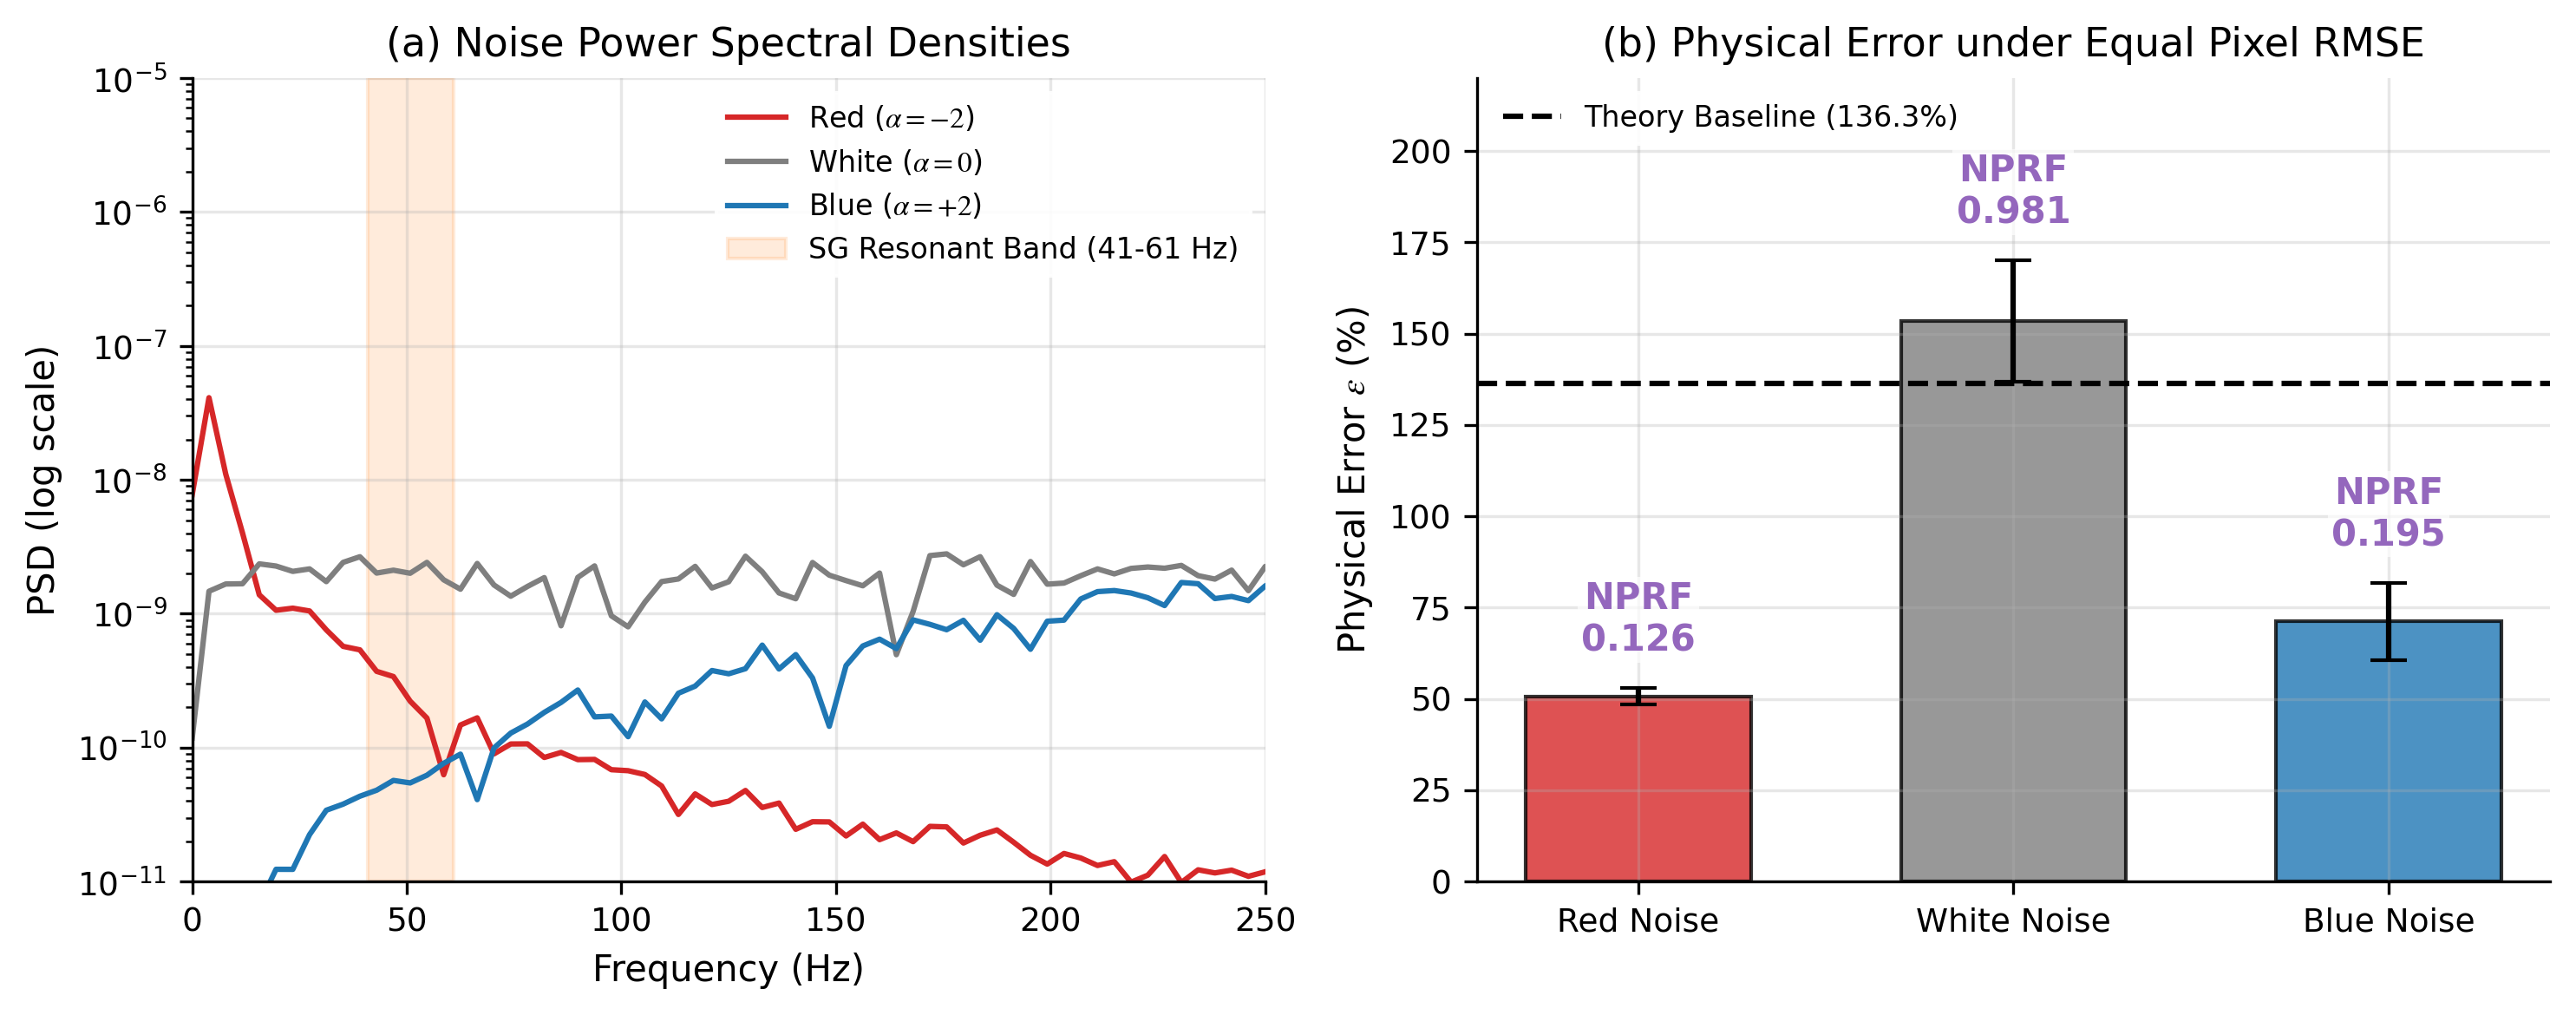
\includegraphics[width=0.8\columnwidth]{1.png}
    \caption{Spectral-adversarial vulnerability. (a) PSDs for red/white/blue noise; SG resonant band shaded. (b) Under identical pixel RMSE, physical error differs by 3.03$\times$; NPRF correctly ranks risk.}
    \label{fig:fig1}
\end{figure}

\subsection{Experiment 2: Complementary Diagnostics}

\textbf{Amplitude-dominated regime} ($\sigma_{\text{px}} \in [0.0005, 0.005]$, $\alpha \in [-2, 2]$, $n=500$): pixel RMSE varies together with spectral shape. \textbf{Amplitude-blind regime} ($\sigma_{\text{px}} = 0.001$ fixed, $\alpha \in [-2.5, 2.5]$, $n=300$): only spectral shape varies.

\begin{center}
    \scriptsize\setlength{\tabcolsep}{3.5pt}
    \begin{tabular}{lcc}
        \toprule
        \textbf{Regime} & \textbf{Metric} & \textbf{Spearman $\bm{\rho}$} \\
        \midrule
        \multirow{2}{*}{Amplitude-dominated ($n{=}500$)} & $\pxrmse$ & $\mathbf{0.813}$ ($p<0.001$) \\
         & $\nprf$ & $0.463$ ($p<0.001$) \\
        \midrule
        \multirow{2}{*}{Amplitude-blind ($n{=}300$)} & $\pxrmse$ & N/A (held constant) \\
         & $\nprf$ & $\mathbf{0.968}$ ($p<0.001$) \\
        \bottomrule
    \end{tabular}
    \\[0.2pt]
    {\scriptsize \textbf{Table 2:} RMSE performs best in amplitude-dominated region ($\rho=0.813$); NPRF takes over in amplitude-blind region ($\rho=0.968$). Both indispensable.}
\end{center}

\begin{figure}[htbp]
    \centering
    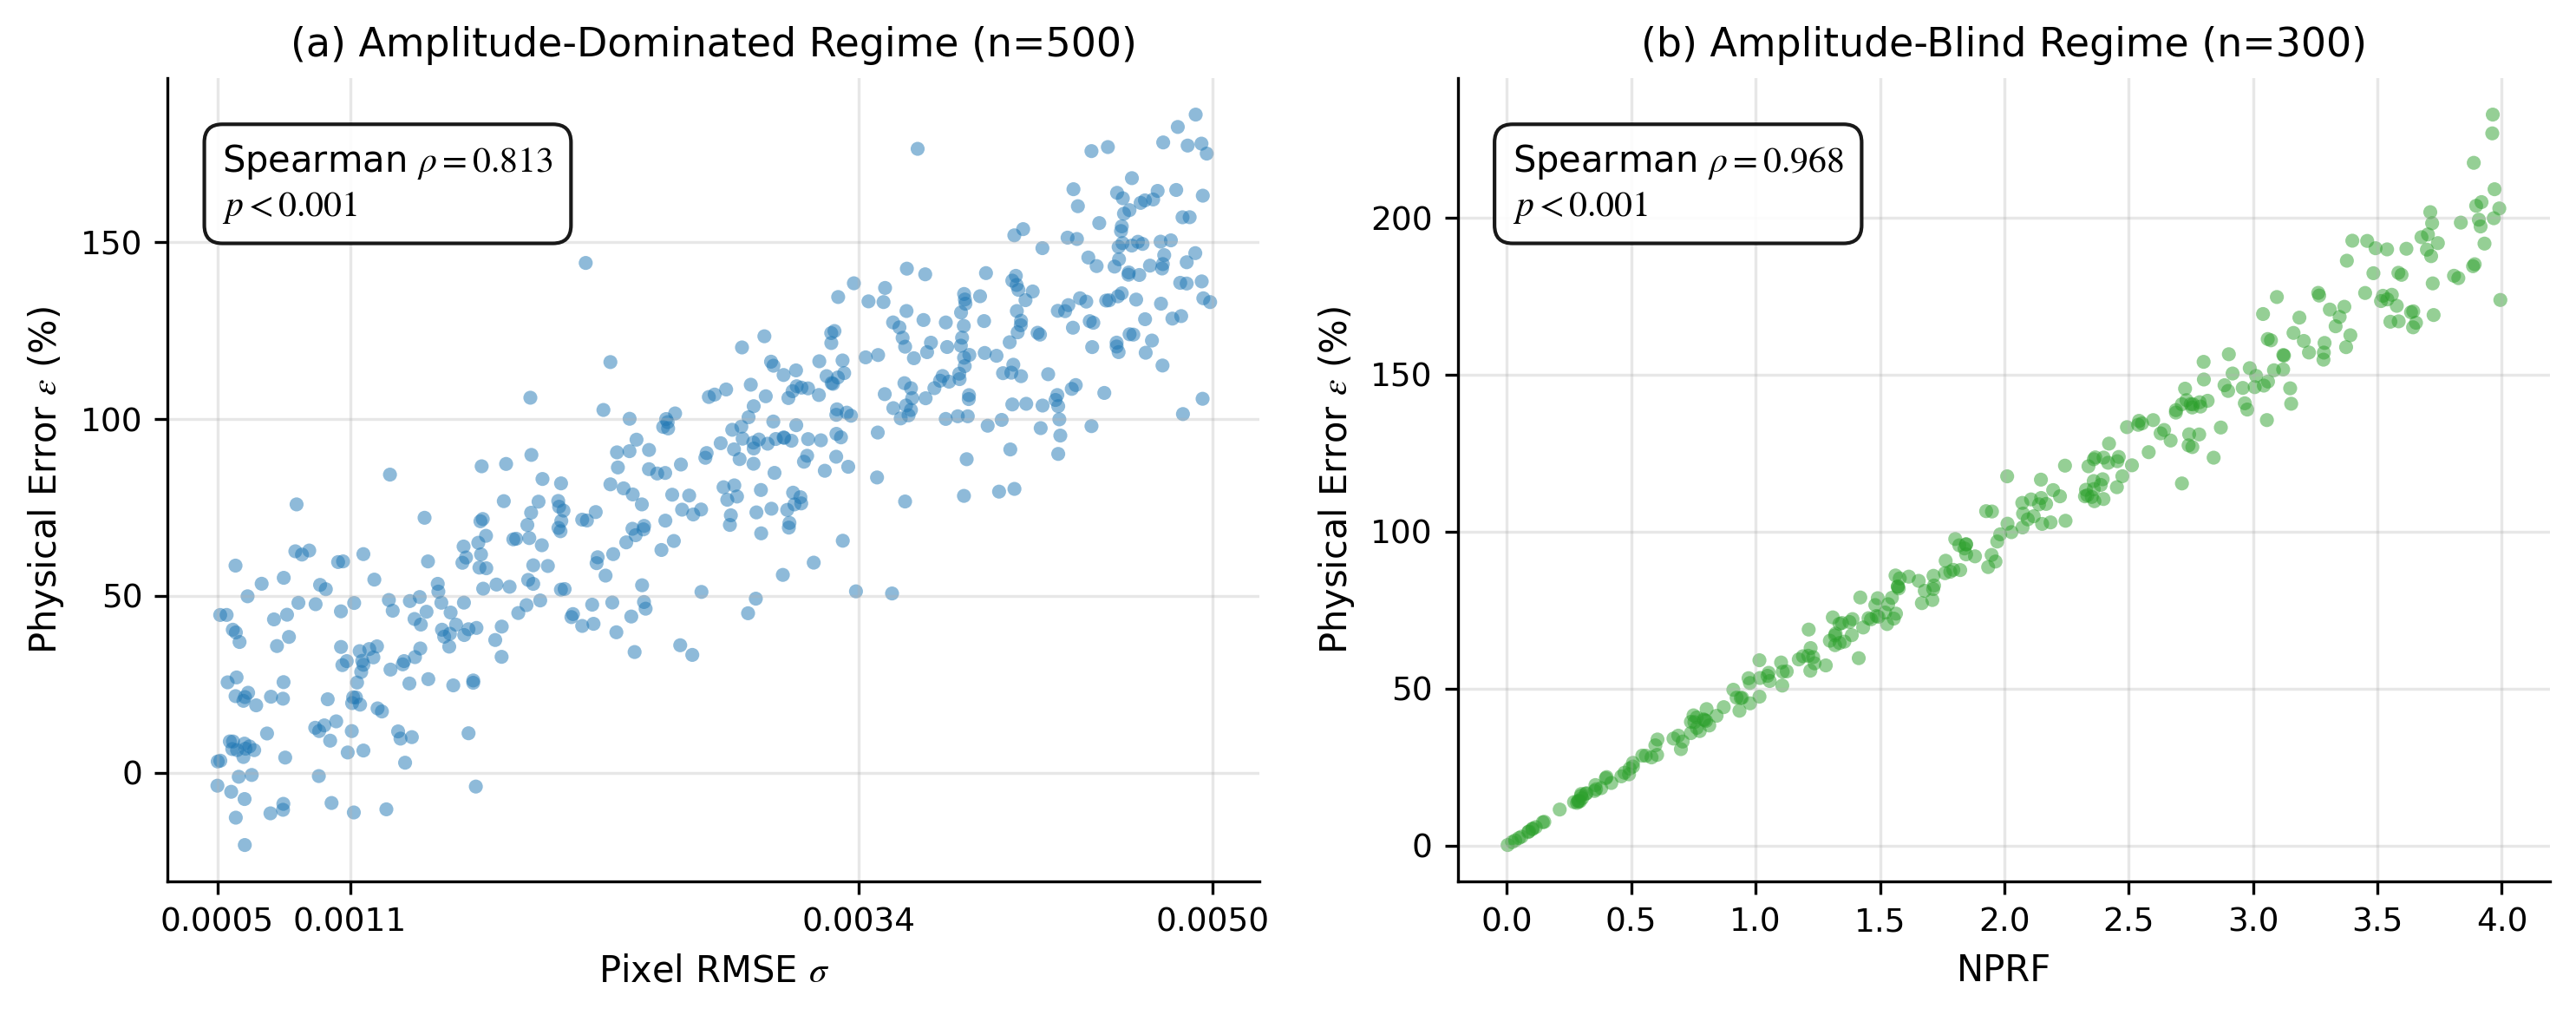
\includegraphics[width=0.8\columnwidth]{2.png}
    \caption{Complementary diagnostics. (a) Amplitude-dominated: RMSE correlates strongly ($\rho=0.813$). (b) Amplitude-blind: NPRF independently ranks physical error ($\rho=0.968$).}
    \label{fig:fig2}
\end{figure}

\subsection{Experiment 2b: NPRF Early-Warning Case Study}

Two denoising models with \textit{identical} pixel RMSE ($\sigma_{\text{px}} = 0.00200$): Model A (low-freq residual, $\alpha=-2$); Model B (resonant-band residual, 55--65 Hz band-pass).

\begin{center}
    \scriptsize\setlength{\tabcolsep}{3.5pt}
    \begin{tabular}{lccc}
        \toprule
        \textbf{Model} & $\bm{\sigma_{\text{px}}}$ & \textbf{NPRF} & $\bm{\physerr}$(\%) \\
        \midrule
        A (low-freq residual) & 0.00200 & 0.113 & 98.7 \\
        B (resonant residual) & 0.00200 & $\mathbf{8.875}$ & $\mathbf{815.3}$ \\
        \bottomrule
    \end{tabular}
    \\[0.2pt]
    {\scriptsize \textbf{Table 3:} Pixel RMSE identical; physical error differs 8.26$\times$; NPRF correctly flags Model B as high-risk.}
\end{center}

\textbf{Key finding:} A practitioner monitoring only pixel RMSE would deem both models equivalent; NPRF reveals an 8.26$\times$ hidden disparity.

\subsection{Experiment 3: MSE Training Spectral Limitations}

\textbf{Setup:} clean signal 10 Hz + 60 Hz (amplitude 1.0). MLP denoisers (64-32, ReLU, Adam, 200 epochs), $n=20$/condition. Test noise: white+blue, $\sigma=0.002$. \textbf{Ablation:} both groups trained with white noise; Group A uses 10 Hz signal only, Group B uses 10 Hz + 60 Hz.

\begin{center}
    \scriptsize\setlength{\tabcolsep}{2.5pt}
    \begin{tabular}{lccc}
        \toprule
        \textbf{Training noise} & $\bm{\pxrmse}$ & $\nprf$ & $\bm{\physerr}$(\%) \\
        \midrule
        Red noise & $0.00209_{\pm0.00039}$ & $3.701_{\pm1.767}$ & $510.5_{\pm194.0}$ \\
        White noise & $0.00220_{\pm0.00146}$ & $2.479_{\pm1.046}$ & $429.3_{\pm267.1}$ \\
        Blue noise & $0.00196_{\pm0.00052}$ & $2.590_{\pm1.273}$ & $394.7_{\pm147.7}$ \\
        \midrule
        Zero predictor & $1.001$ & $5.731$ & $281219$ \\
        \bottomrule
    \end{tabular}
    \\[0.2pt]
    {\scriptsize \textbf{Table 4:} Kruskal-Wallis: $H=5.775$, $p=0.056$. After Bonferroni correction ($\alpha=0.0167$) \textbf{none significant}. Post-hoc power $\approx0.35$; \textbf{marginal directional evidence}; $n\geq60$/group needed. Ablation (10 Hz only vs.\ 10+60 Hz): NPRF $1.167\to2.479$, 2.12-fold ($p=0.000042$, Cohen's $d=1.558$). Signal-type blind-spot is dominant causal driver.}
\end{center}

\textbf{Key findings:} \textbf{First,} models learn denoising ($\pxrmse$ falls $\sim500$-fold). \textbf{Second,} training-noise effects \textit{not} statistically significant after correction. \textbf{Third,} all models have NPRF $>1.0$---dual blind-spots: noise-type (blue-trained: 2.590 vs.\ baseline 0.195) and signal-type (60 Hz within resonant band). MSE training alone does not confer spectral immunity; it must be introduced externally.

\begin{figure}[htbp]
    \centering
    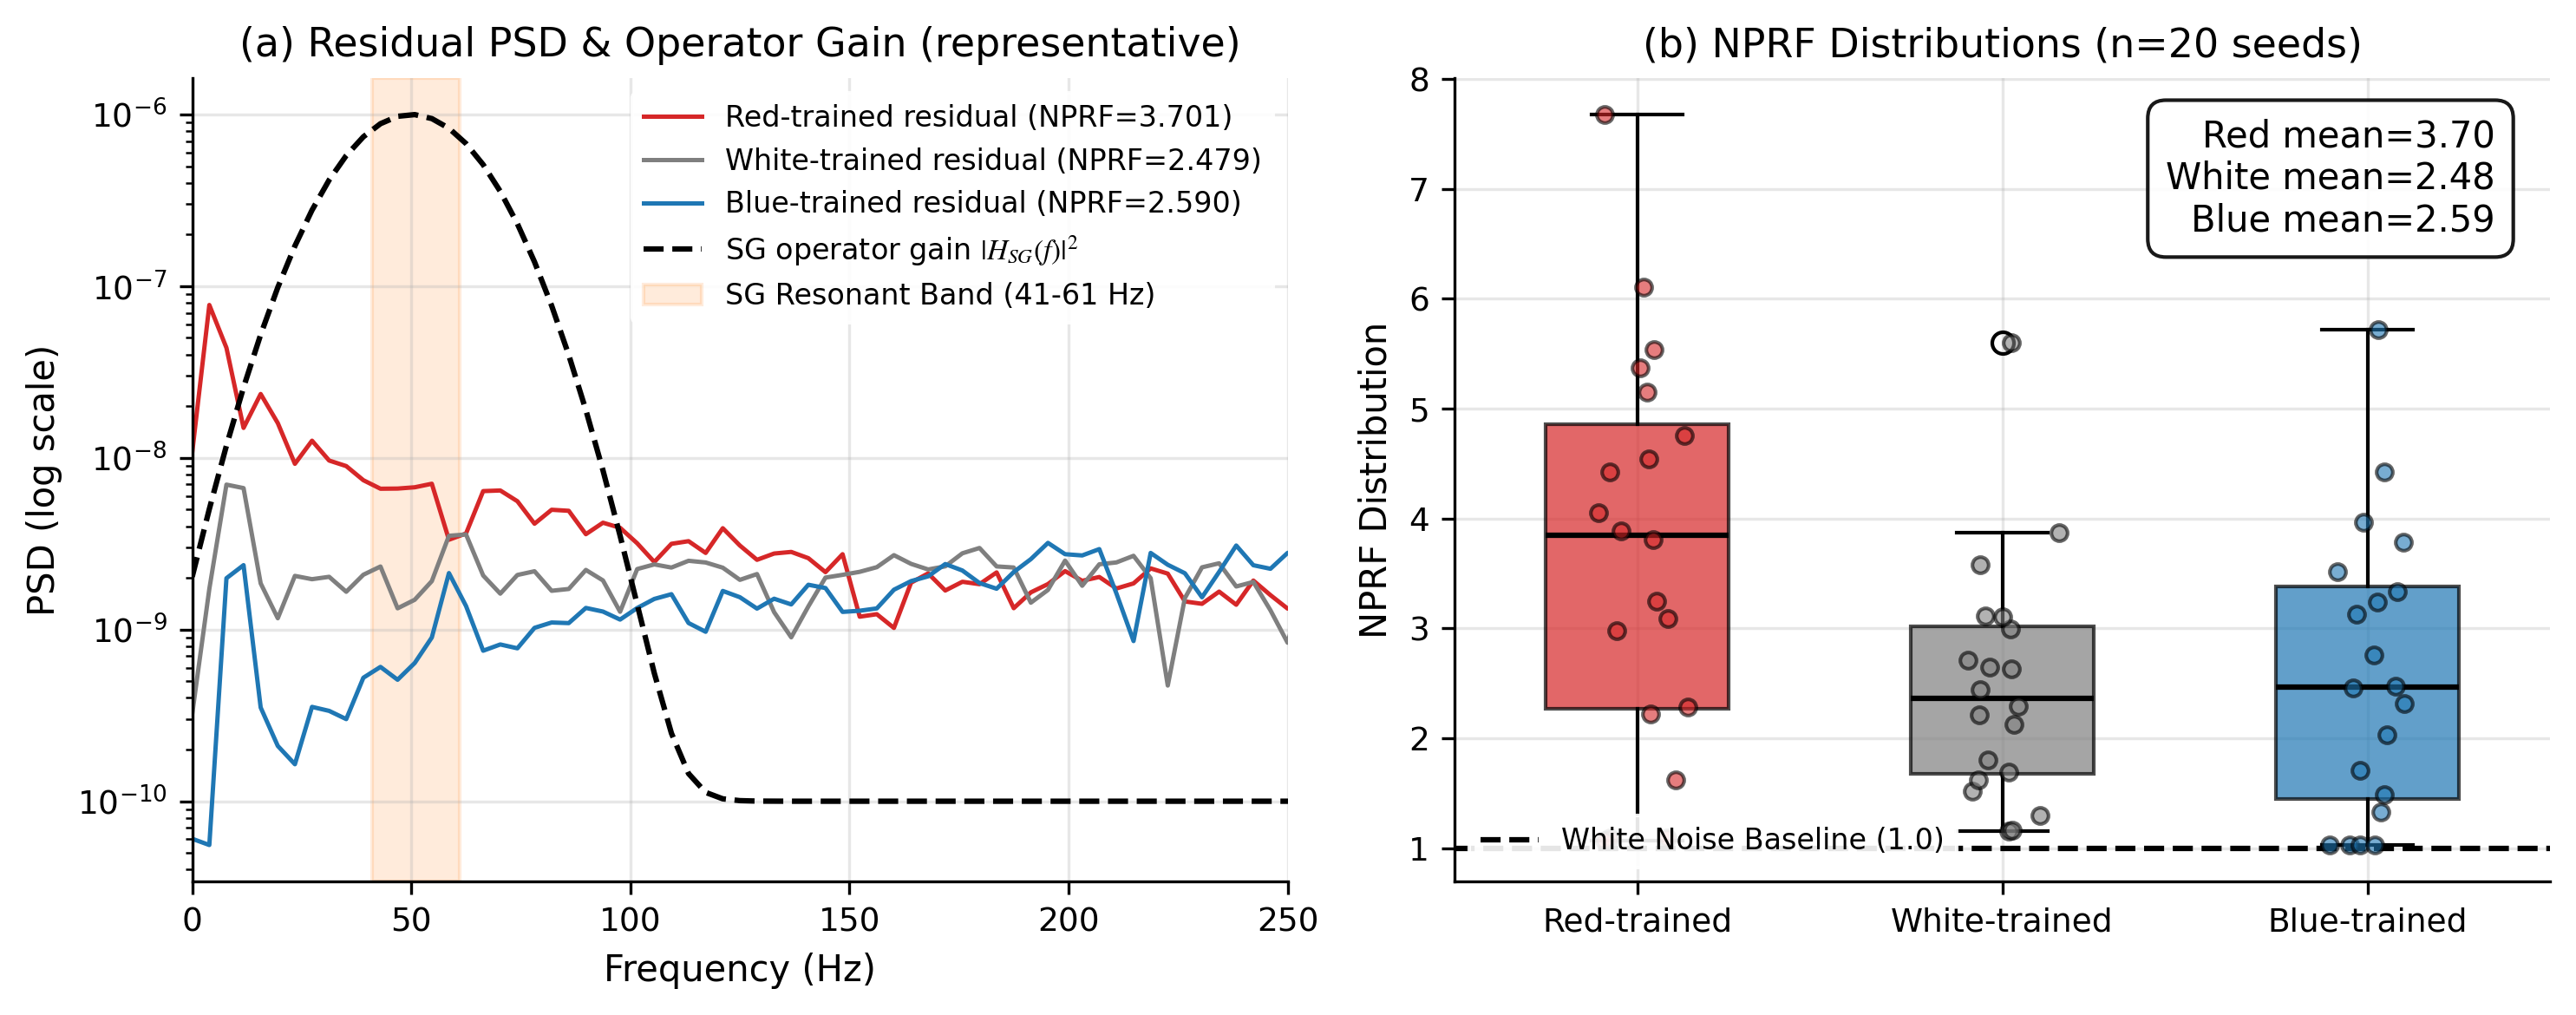
\includegraphics[width=0.8\columnwidth]{3.png}
    \caption{Spectral blind-spots of standard MSE training. (a) Residual PSDs (seed-0); red-trained model leaves resonant-band energy. (b) NPRF distributions ($n=20$); all exceed baseline 1.0.}
    \label{fig:fig3}
\end{figure}

\subsection{Experiment 3b: Post-hoc Spectral Reshaping as Remedy}

Training-time spectral regularization proved numerically unstable (NPRF is a ratio metric whose gradient diverges as $\sigma_{\text{px}}\to0$; resonant-band penalty conflicts with 60 Hz signal preservation). We adopt \textbf{post-hoc spectral reshaping}: five-stage IIR notch (45/48/51/54/57 Hz, $Q=8.0$) on standard-MSE residuals.

\begin{center}
    \scriptsize\setlength{\tabcolsep}{3.5pt}
    \begin{tabular}{lccc}
        \toprule
        \textbf{Stage} & \textbf{NPRF} & $\bm{\physerr}$(\%) & $\bm{\sigma_{\text{px}}}$ \\
        \midrule
        Before reshaping & $2.412_{\pm0.797}$ & $348.2_{\pm114.9}$ & $0.00174_{\pm0.00035}$ \\
        After reshaping & $\mathbf{1.210_{\pm0.312}}$ & $\mathbf{240.4_{\pm74.9}}$ & $0.00160_{\pm0.00028}$ \\
        \bottomrule
    \end{tabular}
    \\[0.2pt]
    {\scriptsize \textbf{Table 5:} Post-hoc notch filtering reduces NPRF by 49.8\% and physical error by 31.0\% ($p=0.001953$, $n=10$ paired). Pixel RMSE essentially unchanged ($-8.0\%$).}
\end{center}

\textbf{Key:} Spectral immunity without retraining---plug-and-play notch filter reshapes residual spectra. Pixel-RMSE cost negligible ($<10\%$) because notch removes only $4\%$ of bandwidth.

\subsection{Experiment 4: Frequency-Domain Anatomy}

Frequency bands around resonant peak $f_{\text{peak}}=51$ Hz: sub-resonant (0--41 Hz), resonant (41--61 Hz), suppression (61--500 Hz).

\begin{center}
    \scriptsize
    \resizebox{\columnwidth}{!}{%
    \begin{tabular}{lccccc}
        \toprule
        \textbf{Band} & \textbf{BW frac. (\%)} & \textbf{White contrib. (\%)} & \textbf{Blue contrib. (\%)} & \textbf{Efficiency ratio} \\
        \midrule
        Sub-resonant & 8.2 & 15.2 & 0.8 & 1.86 \\
        Resonant & 4.0 & \textbf{42.8} & 5.9 & \textbf{10.70} \\
        Suppression & 87.8 & 42.0 & \textbf{93.3} & 0.48 \\
        \bottomrule
    \end{tabular}%
    }
    \\[0.2pt]
    {\scriptsize \textbf{Table 6:} Efficiency ratio = contribution (\%) / bandwidth fraction (\%), measuring risk concentration per unit bandwidth. Within only 4.0\% fractional bandwidth, the resonant band contributes 42.8\% of integrated physical error for white noise (efficiency ratio 10.70). Blue-noise energy concentrates in suppression band (93.3\%).}
\end{center}

\textbf{Key finding:} Resonant-band risk-efficiency is 10.70$\times$ the full-band average, confirming that spectral-immunity strategies should prioritize resonant-band mitigation.

\subsection{Experiment 5: Engineering Validation}

\textbf{Setup:} 100 non-stationary-noise samples ($\alpha\in[0,2]$, $\sigma\in[0.0020,0.0035]$). A: no filtering; B: Butterworth $f_c=150$ Hz; C: five-stage IIR notch (45/48/51/54/57 Hz, $Q=8.0$).

\begin{center}
    \scriptsize
    \resizebox{\columnwidth}{!}{%
    \begin{tabular}{lccc}
        \toprule
        \textbf{Filter} & $\bm{\physerr}$(\%) & $\nprf$ & \textbf{Pixel RMSE} \\
        \midrule
        A (no processing) & $292.4_{\pm51.0}$ & $0.448_{\pm0.087}$ & $0.00277_{\pm0.00015}$ \\
        B (Butterworth) & $229.7_{\pm36.0}$ & $2.151_{\pm0.431}$ & $0.00097_{\pm0.00010}$ \\
        C (Spectral-Immunity) & $272.3_{\pm45.8}$ & $\mathbf{0.440_{\pm0.094}}$ & $0.00260_{\pm0.00014}$ \\
        \bottomrule
    \end{tabular}%
    }
    \\[0.2pt]
    {\scriptsize \textbf{Table 7:} Mann-Whitney U: A vs B $p<0.001$; A vs C $p=0.0011$. Butterworth raises NPRF +380.0\%: $f_c=150$ Hz suppresses out-of-band energy far more than resonant-band energy, causing $\sigma_{\text{px}}^2$ (denominator) to fall faster than the weighted numerator. Notch preserves NPRF near baseline. Ratio-method prediction deviation: 2.4\%.}
\end{center}

\begin{figure}[htbp]
    \centering
    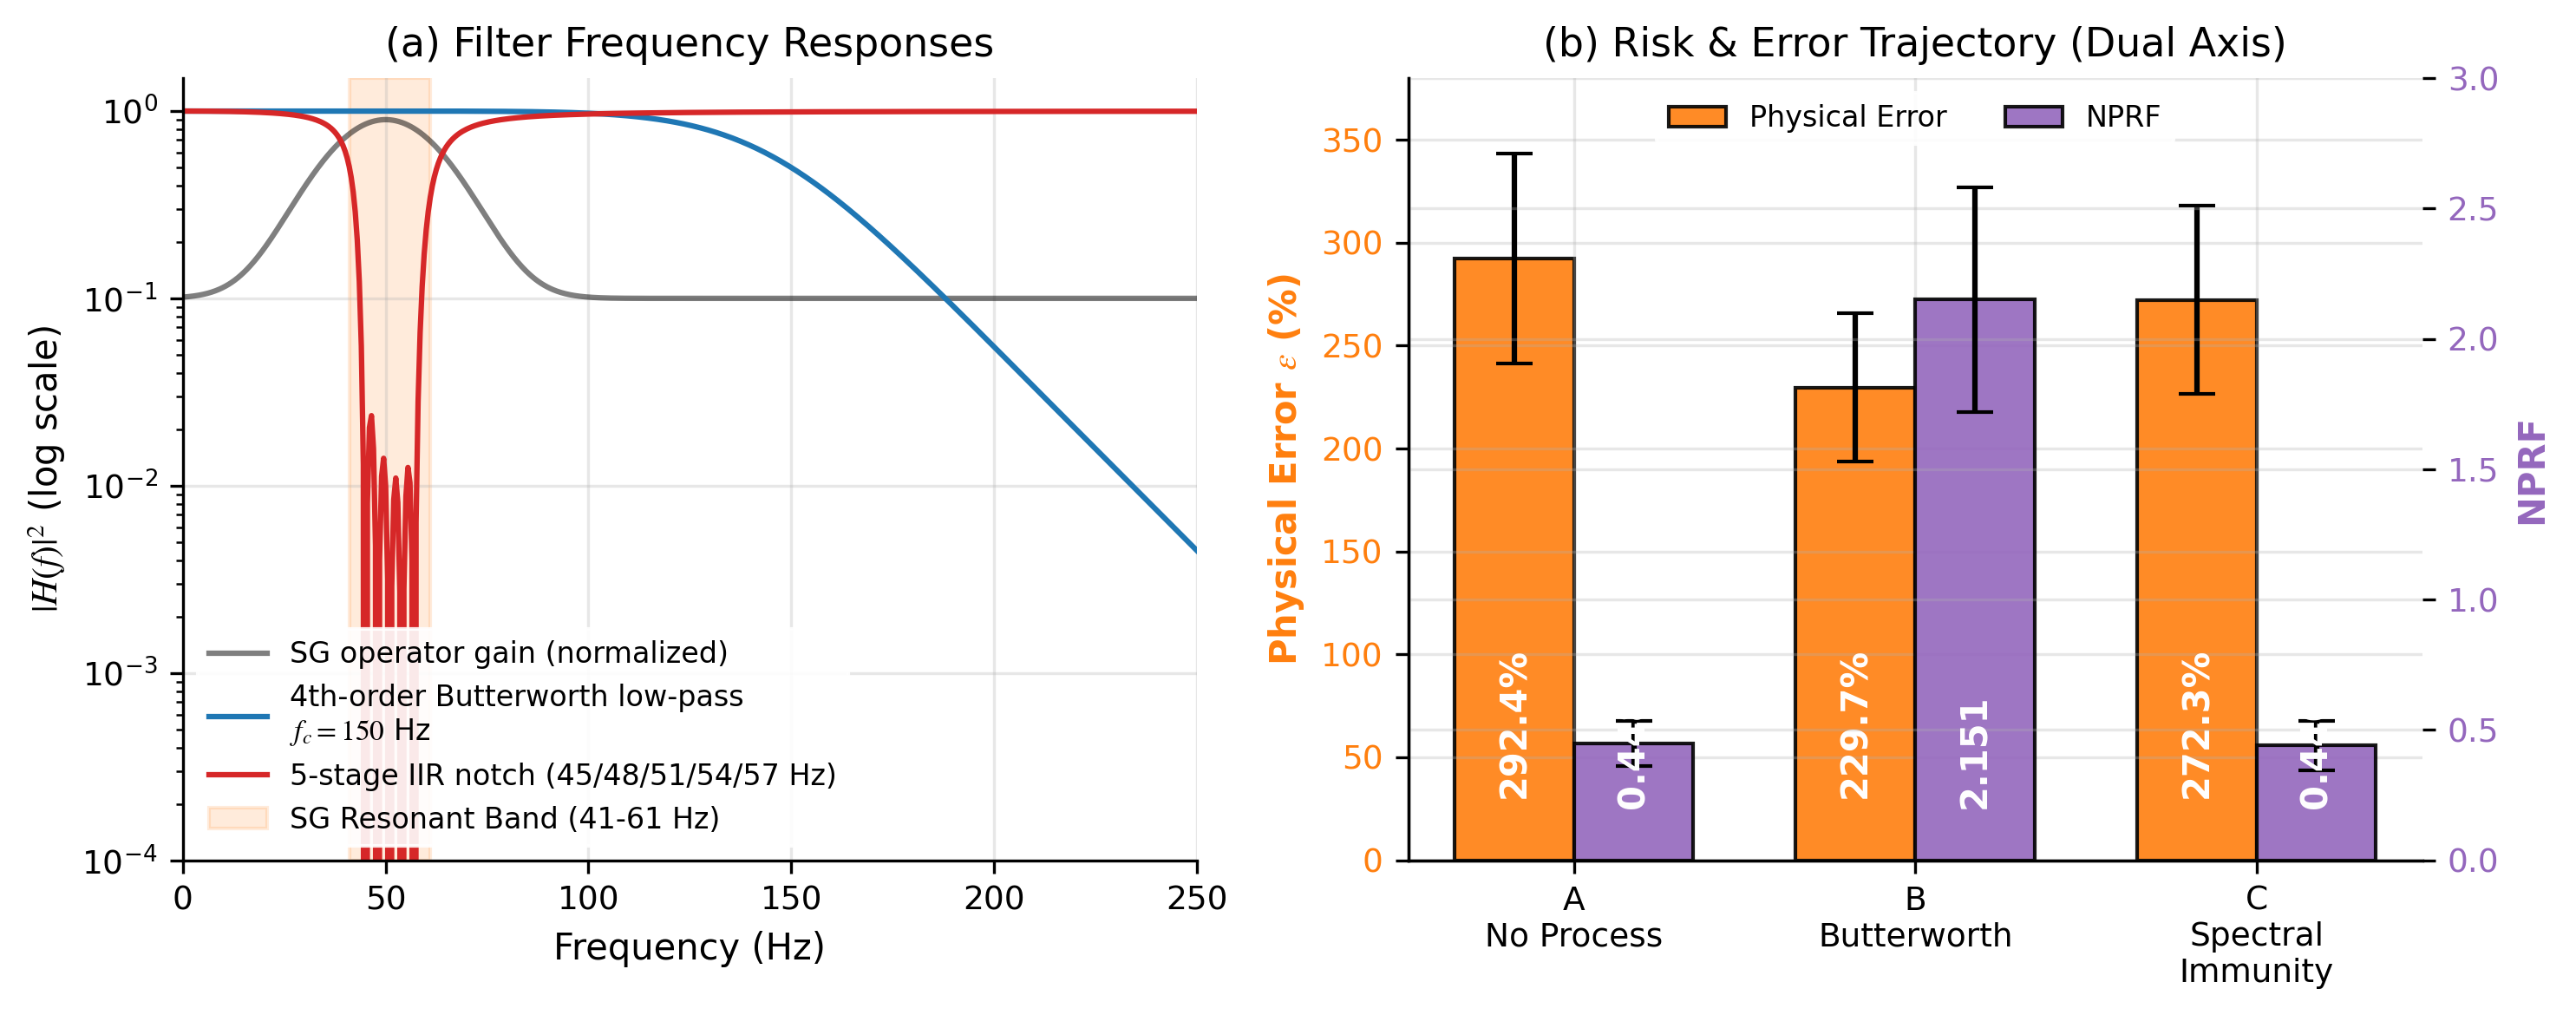
\includegraphics[width=0.8\columnwidth]{4.png}
    \caption{Engineering validation. (a) Filter responses vs.\ SG resonant band; notch attenuates resonant energy, Butterworth does not. (b) NPRF vs.\ physical error ($n=100$).}
    \label{fig:fig4}
\end{figure}

\subsection{Experiment 6: Real-World Basketball Projectile (No Statistical Claims)}

\textbf{Setup:} DJI Action (48 fps), 53 frames manual tracking. Ball diameter 0.246 m $\approx$ 40 px, scale $6.15\times10^{-3}$ m/px. 2D projectile: $x(t)$ linear, $y(t)$ quadratic.

\begin{center}
    \scriptsize\setlength{\tabcolsep}{3.5pt}
    \begin{tabular}{lcc}
        \toprule
        \textbf{Quantity} & \textbf{Value} & \textbf{Note} \\
        \midrule
        $v_{0x}$ & 5.20 m/s & $R^2=0.9974$ \\
        $a_y$ & $-11.29$ m/s$^2$ & 15.2\% bias from $g$ \\
        $\sigma_x$ / $\sigma_y$ & 84.9 / 67.0 mm & Tracking noise \\
        Frame-wise phys.\ error & 75.3\% & SG instantaneous $a$ \\
        NPRF & 0.177 & Concept only \\
        \bottomrule
    \end{tabular}
    \\[0.2pt]
    {\scriptsize \textbf{Table 8:} Bias sources: calibration ($\pm5\%$), lens distortion, air resistance (0.3\% of $g$). $N=53$: no CI possible; NPRF serves as workflow demonstration only. Pipeline executes end-to-end in $<$1 s.}
\end{center}

% ==================== 4. Limitations and Deployment ====================
\section{Limitations and Deployment}

\subsection{Limitations}

\textbf{Linear-operator assumption} may break for strongly non-linear operators. \textbf{Calibration dependency:} black-box pipelines require numerical perturbation. \textbf{Statistical power:} Experiment 3 marginal ($p=0.056$, power$\approx0.35$); ablation sufficient ($p=0.000042$). \textbf{Signal-noise overlap:} notch filters attenuate genuine 60 Hz signal. \textbf{Welch leakage:} screening only for $N<200$. \textbf{PGTS-to-real-world gap:} quantitative results inside PGTS only. NPRF complements UQ: UQ asks ``how uncertain?'' NPRF asks ``how physically dangerous?''

\subsection{Deployment}

\textbf{(1) Spectral health check for AI-for-Science:} NPRF after every prediction, no costly DFT validation. \textbf{(2) Vision-based tracking:} trigger ``slow-down'' when NPRF$>2.0$. \textbf{(3) Quality-gating:} mark low-confidence when NPRF$>1.5$--$2.0$, no gold-standard annotations required\cite{ardila2019}.

\subsection{Future Work}

Spectral adversarial training (resonant-band energy penalty, squared norm, avoiding ratio-gradient instability). Adaptive notch filters. Non-linear extensions (Volterra series). NPRF asymptotic theory. Realistic-scenario validation. Ideal rectangular-notch upper bound for Spectral-Immunity filter benchmarking.

% ==================== 5. Conclusion ====================
\section{Conclusion}

Pixel-RMSE suffers structural failure within physical-derivation pipelines: identical pixel error magnitudes produce physical errors differing 3.03$\times$ (general) to 8.26$\times$ (adversarial). This paper presents the first spectral-theoretic solution, shifting from ``pixel-based trust'' to ``spectral-based trust.''

Core contributions: (1) spectral sufficiency theorem (Thm.\ \ref{thm:sufficiency}); (2) NPRF requiring no physical ground truth (Eq.\ \ref{eq:nprf_def}); (3) dual RMSE+NPRF paradigm; (4) early-warning (8.26$\times$ disparity); (5) post-hoc remedy (NPRF $-49.8\%$, $p=0.002$); (6) counter-intuitive Butterworth finding (+380.0\% NPRF); (7) dual MSE blind-spots with ablation ($p=0.000042$, $d=1.558$); (8) real-world proof-of-concept.

\begingroup
\scriptsize
\textbf{Boundary statement:} Proves: (1) pixel-RMSE structural failure under operator resonance; (2) NPRF feasibility; (3) MSE spectral blind-spots; (4) post-hoc reshaping efficacy in PGTS. Does \textbf{not} prove: (a) NPRF validity for arbitrary non-linear operators; (b) filter generalizability beyond PGTS; (c) training-noise-type significance ($p=0.056$, power$\approx0.35$).
\endgroup

\vspace{0.5pt}

Every AI Scientist that derives physical quantities from observational data is, knowingly or not, making a bet about the spectral flatness of its residual errors. This paper shows that bet is often lost. The \textbf{Spectral Vaccine}---NPRF diagnosis plus post-hoc Spectral-Immunity filtering---provides the first deployable immune response. The plug-and-play nature of NPRF---no ground truth, minimal overhead, offline calibration---makes it a candidate for infrastructure. \textbf{Future AI-Scientists need not only powerful reasoning, but also an intrinsic immune system---autonomously asking, before every output: is my result physically credible?}

\vspace{0.3pt}
{\scriptsize\noindent\textbf{Acknowledgements:} We thank Supervisor Wei Teng, head teachers Ms. Minglu Zhang and Mr. Zheng Niu, and grade director Ms. Qian Ren for their support. Code: \texttt{https://github.com/RosslynKira/spectral-immunity}}

% ==================== References ====================
\begingroup
\scriptsize
\setlength{\itemsep}{0pt}
\setlength{\parsep}{0pt}
\renewcommand{\baselinestretch}{0.68}
\begin{thebibliography}{99}

\bibitem{abramson2024}
J.~Abramson, J.~Adler, J.~Dunger, et al.
\newblock Accurate structure prediction of biomolecular interactions with AlphaFold 3.
\newblock \textit{Nature}, 630:493--500, 2024.

\bibitem{merchant2023}
A.~Merchant, S.~Batzner, S.~S.~Schoenholz, et al.
\newblock Scaling deep learning for materials discovery.
\newblock \textit{Nature}, 624:80--85, 2023.

\bibitem{lam2023}
R.~Lam, A.~Sanchez-Gonzalez, M.~Willson, et al.
\newblock Learning skillful medium-range global weather forecasting.
\newblock \textit{Science}, 382:1416--1421, 2023.

\bibitem{savitzky1964}
A.~Savitzky and M.~J.~E.~Golay.
\newblock Smoothing and differentiation of data by simplified least squares procedures.
\newblock \textit{Analytical Chemistry}, 36(8):1627--1639, 1964.

\bibitem{welch1967}
P.~D.~Welch.
\newblock The use of fast Fourier transform for the estimation of power spectra: a method based on time averaging over short, modified periodograms.
\newblock \textit{IEEE Transactions on Audio and Electroacoustics}, 15(2):70--73, 1967.

\bibitem{brillinger2001}
D.~R.~Brillinger.
\newblock \textit{Time Series: Data Analysis and Theory}. SIAM, 2001.

\bibitem{kasdin1995}
N.~J.~Kasdin.
\newblock Discrete simulation of colored noise and stochastic processes and $1/f^\alpha$ power law noise generation.
\newblock \textit{Proceedings of the IEEE}, 83(5):802--827, 1995.

\bibitem{burger2020}
B.~Burger, P.~M.~Maffettone, V.~V.~Gusev, et al.
\newblock A mobile robotic chemist.
\newblock \textit{Nature}, 583:237--241, 2020.

\bibitem{xu2019}
Z.-Q.~J.~Xu, Y.~Zhang, and Y.~Xiao.
\newblock Training behavior of deep neural network in frequency domain.
\newblock In \textit{Neural Information Processing, ICONIP 2019}, LNCS 11953, pp.~264--274, Springer, 2019.

\bibitem{ardila2019}
D.~Ardila, A.~P.~Kiraly, S.~Bharadwaj, et al.
\newblock End-to-end lung cancer screening with three-dimensional deep learning on low-dose chest computed tomography.
\newblock \textit{Nature Medicine}, 25(6):954--961, 2019.

\bibitem{rahaman2019}
N.~Rahaman, A.~Baratin, D.~Arpit, et al.
\newblock On the spectral bias of neural networks.
\newblock \textit{Proceedings of the 36th International Conference on Machine Learning}, PMLR 97:5301--5310, 2019.

\bibitem{kendall2017}
A.~Kendall and Y.~Gal.
\newblock What uncertainties do we need in Bayesian deep learning for computer vision?
\newblock \textit{Advances in Neural Information Processing Systems 30}, 2017.

\bibitem{lakshminarayanan2017}
B.~Lakshminarayanan, A.~Pritzel, and C.~Blundell.
\newblock Simple and scalable predictive uncertainty estimation using deep ensembles.
\newblock \textit{Advances in Neural Information Processing Systems 30}, 2017.

\bibitem{tancik2020}
M.~Tancik, P.~P.~Srinivasan, B.~Mildenhall, et al.
\newblock Fourier features let networks learn high frequency functions in low dimensional domains.
\newblock \textit{Advances in Neural Information Processing Systems 33}, 2020.

\bibitem{ronen2019}
R.~Basri, D.~Jacobs, Y.~Kasten, and S.~Kritchman.
\newblock The convergence rate of neural networks for learned functions of different frequencies.
\newblock \textit{Advances in Neural Information Processing Systems 32}, pp.~4761--4771, 2019.

\end{thebibliography}

\endgroup

\end{document}